% Project Proposal Document
\documentclass[final]{cmpreport}
\makeatletter
\input{t1pcr.fd}
\makeatother
\setlength{\footnotesep}{3ex}
\title{\Codex: A Progressive Web App in React for table-top role-playing games}
\author{Christopher Alastair Irvine}
\registration{100036248}
\supervisor{Dr Katharina Huber}
\ccode{CMP-6013Y}
\summary{This project is the tits and here's why...}
\acknowledgements{
	I would like to thank Dr Katharina Huber for taking on the supervision of this project, 
	and guiding me towards success. Additionally I would like to thank Wizards of the Coast 
	for their generosity and kindness in allowing the use of their Intellectual Property for this project.
}
\usepackage{rotating}
\newcommand{\ueacmp}{UEA School of Computing Sciences}
\newcommand{\WotC}{Wizards of the Coast}
\newcommand{\dnd}{D\&D}
\newcommand{\sem}{Software Engineering Model}
\newcommand{\sems}{Software Engineering Models}
\newcommand{\Codex}{\textsc{Codex}}
\newcommand{\AgileSolo}{\emph{Agile Solo}}
% EOF Preamble and Macros
	
% BOF Document
\begin{document}	
	% BOF Introduction
	\section{Introduction} \label{sec:introduction}
	hello there
	
	\section{What is \Codex?} \label{sec:what-codex}
	\Codex \ was a project that has two components. The first, produce a progressive web app built in ReactJS that was developed using a single developer Agile software engineering methodology, the second component was to evaluate the quality of that methodology. By the end of this section we will have an appreciation of the \Codex \ app, in terms of both context and purpose (see Sections \ref{sec:context} and \ref{sec:purpose} respectively).
	
		\subsection{Context} \label{sec:context}
		The \Codex \ an app was based around the popular tabletop role-playing game known as Dungeons and Dragons (\dnd), created and published by \WotC. This game, and the principles that bring the game to life, drove the requirements which formed the basic structure of the \Codex \ app. Therefore, in order to understand the functionality, principle and importance of the \Codex \ app, we must first gain an understanding of \dnd. 
		
		The author of this paper has multiple years of experience with \dnd, both as a \emph{Player} and \emph{Dungeon Master} (DM). The \Codex \ app began as a personal project for the author of this paper, which grew into a tool to evaluate a single developer Agile software engineering methodology. 
		
			\subsubsection{What is Dungeons and Dragons?} \label{sec:what-dnd}
			The game of \dnd, at time of writing, was a popular tabletop role-playing game where a group of friends engage in a grand fantasy adventure powered by a narrative (\cite{DnDOriginal}, \cite{DnDHistory}). The story would be divided into manageable blocks of time known as \emph{sessions}. Each session may take between two and four hours to run, however this is not strictly enforced and is decided by the group of players. The events of each session, and the larger campaign, was created and controlled by a player known as the \emph{Dungeon Master} (DM) (for more details on DMs please see Section \ref{sec:dm-vs-player}). However, the campaign would not always occur as written. The players, who were clueless as to the next plot in the campaign, might take the story in an entirely different direction several times a session. The DM would have to react to these unexpected inputs and redraw the narrative during each session, or attempt to guide the players subtly back on track \citep{PlayerHandbook}. 
			
			Whilst it was possible for DMs to purchase pre-written campaigns, published either by experienced DMs or \WotC, many DMs would take it upon themselves to create their own worlds in which the campaign would occur or alter the pre-written campaigns to suit the needs of the group. For every game of \dnd \ was inherently different from each other, including those following the same campaign book. Because of this difference it was hard to estimate how many sessions a campaign might take. 
			
			The players would form an entity known as the \emph{party}, that would consist of the characters that the players embodied for the duration of the campaign. Each player controls one character, known as the \emph{player character}, within the party. The party would serve as the groups device in how they interact with the world, this is true for the DM who would not embody one character, but every other character within the world. These characters would be referred to ask \emph{non-player characters} and would include both allies and enemies of the party. For that reason, the external perception of the \dnd \ might be that the players were against the DM. Nothing could be further from the truth, as it was the relationship that existed between the players and the DM that would shape the outcome of the campaign \citep{DnDPeople}.
			
			\begin{figure}[h] \label{fig:dnd-equipment}
				\begin{subfigure}{0.5\textwidth}
					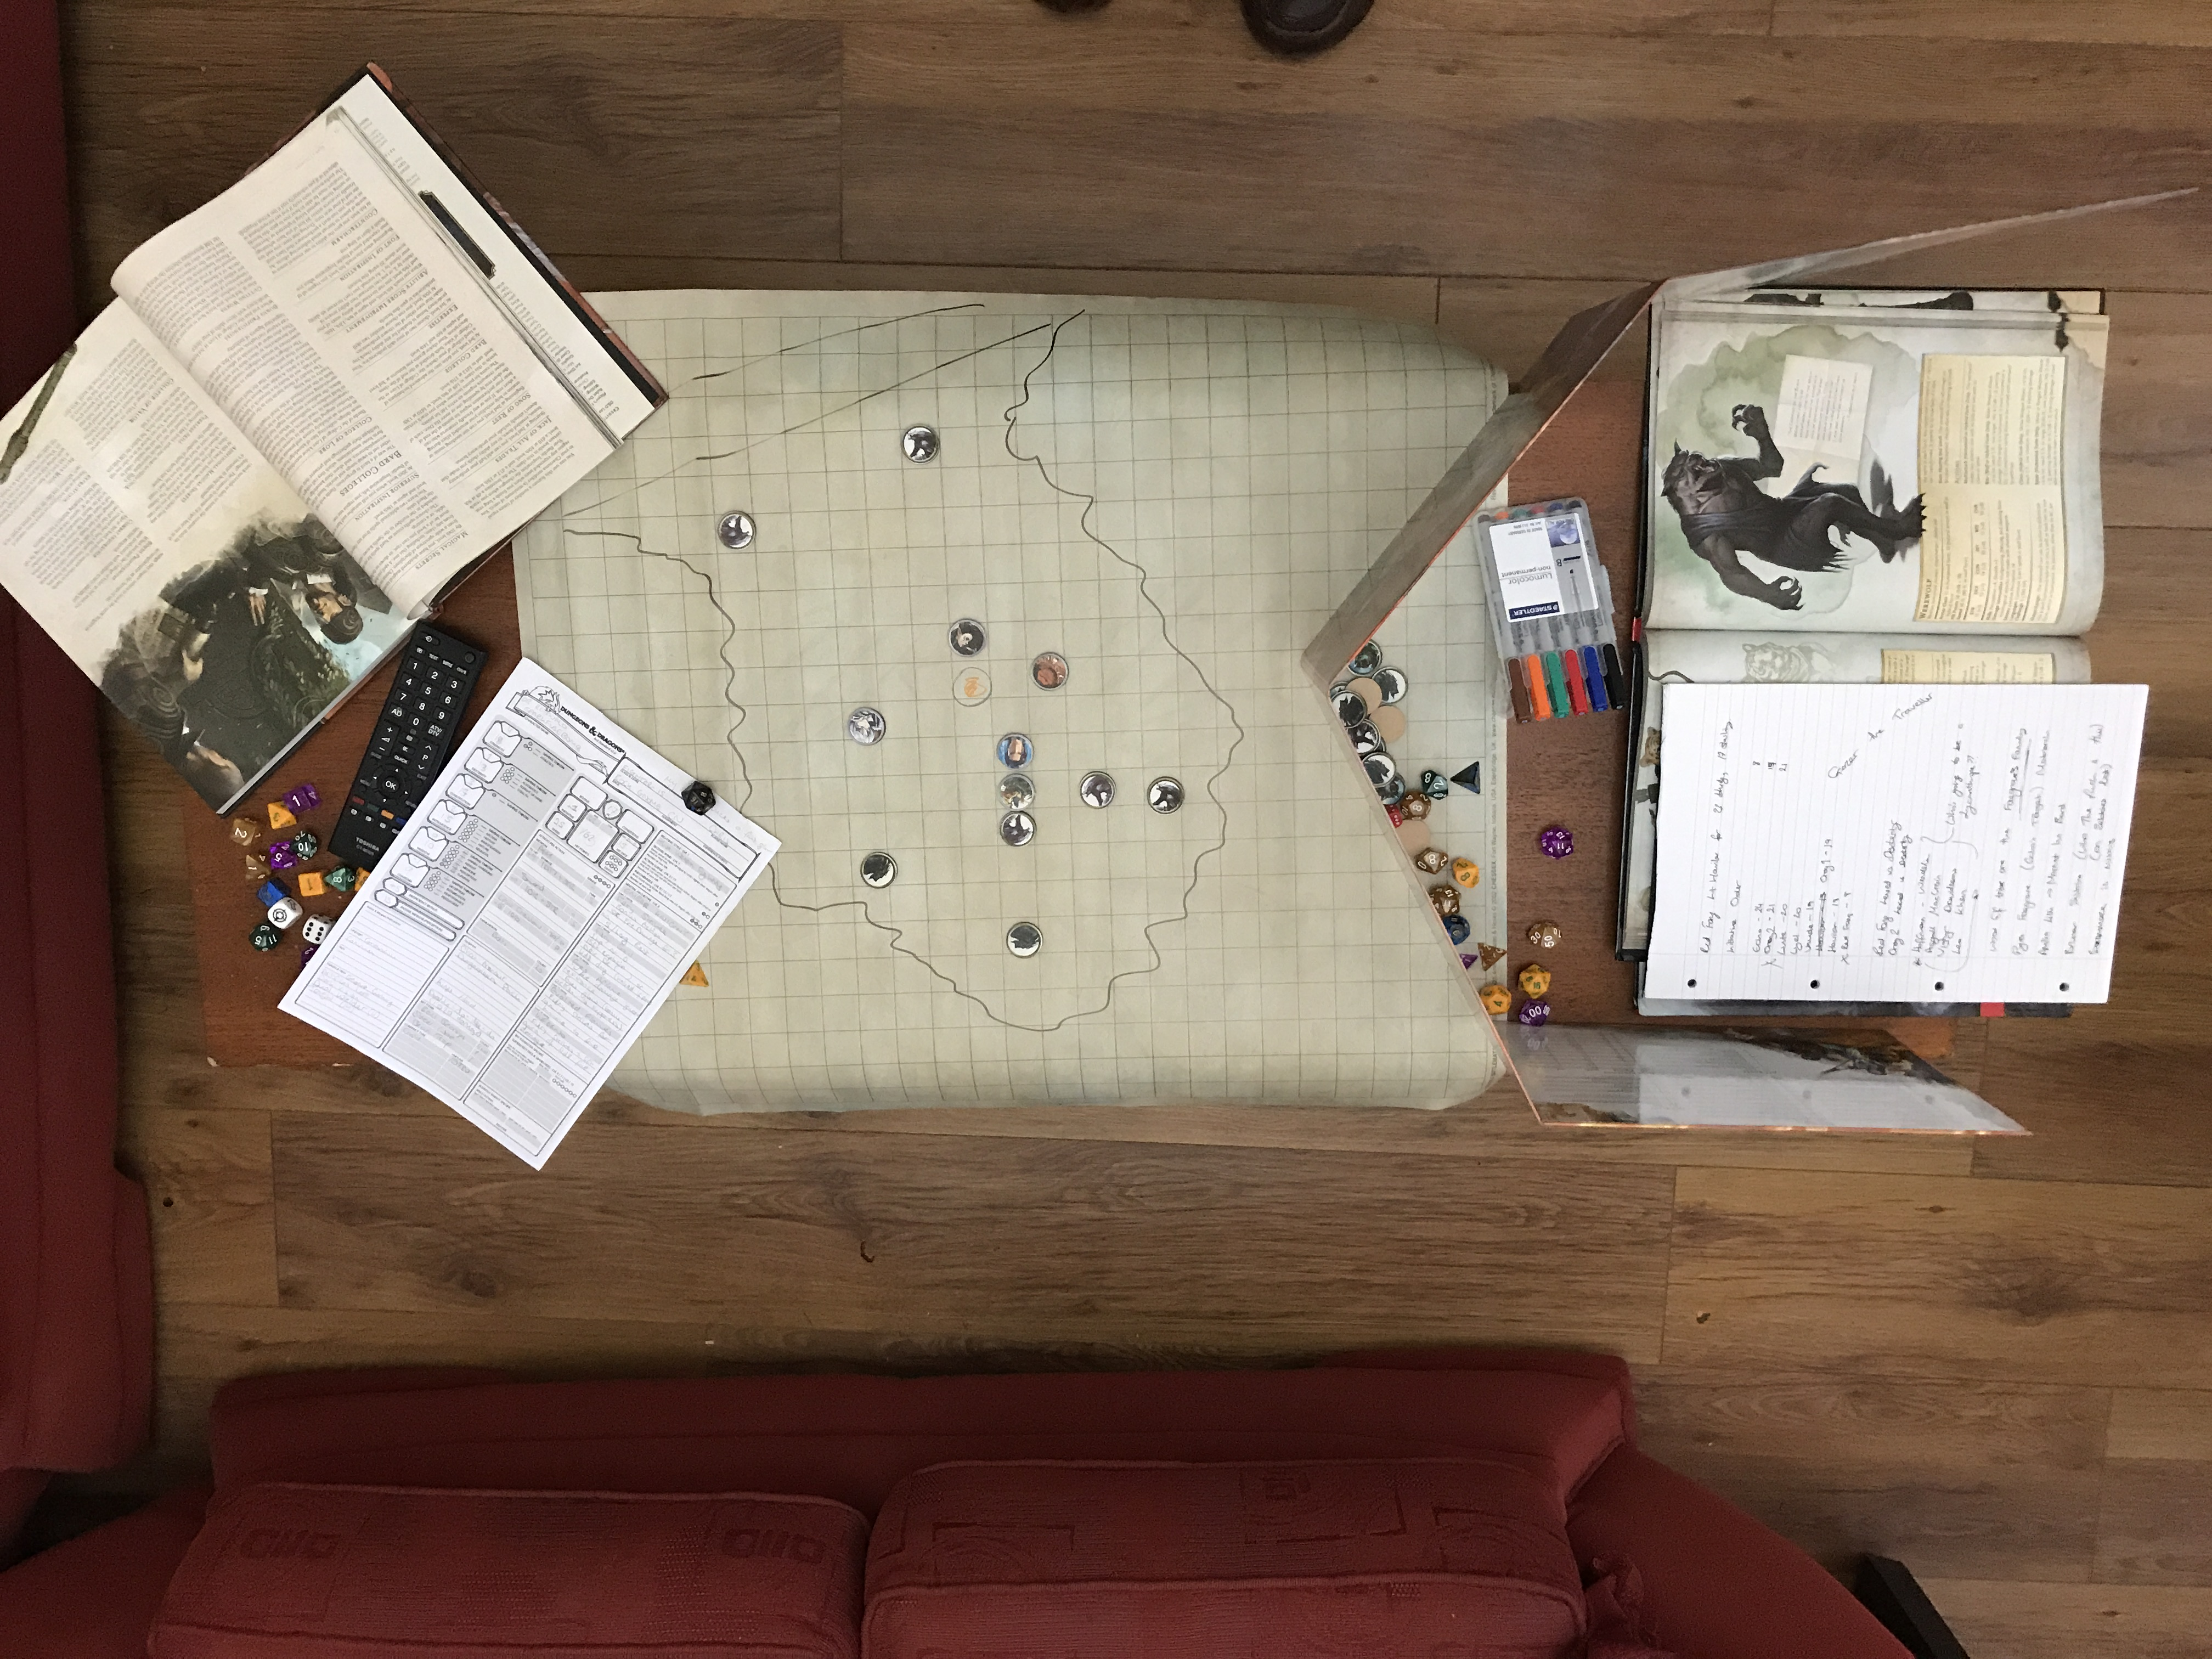
\includegraphics[width=\linewidth, height=5cm, angle=180]{DnD_Live.jpg}
					\caption{A typical \dnd \ set up. From left to right: DM note pad on top of a couple of official \WotC \ core books (\emph{Monster Manual} shown), set of die, battle mat and tokens, a player character sheet, player's set of die and the \WotC \ \emph{Players Handbook}} \label{fig:DnDLive}
				\end{subfigure}
				\begin{subfigure}{0.5\textwidth}
					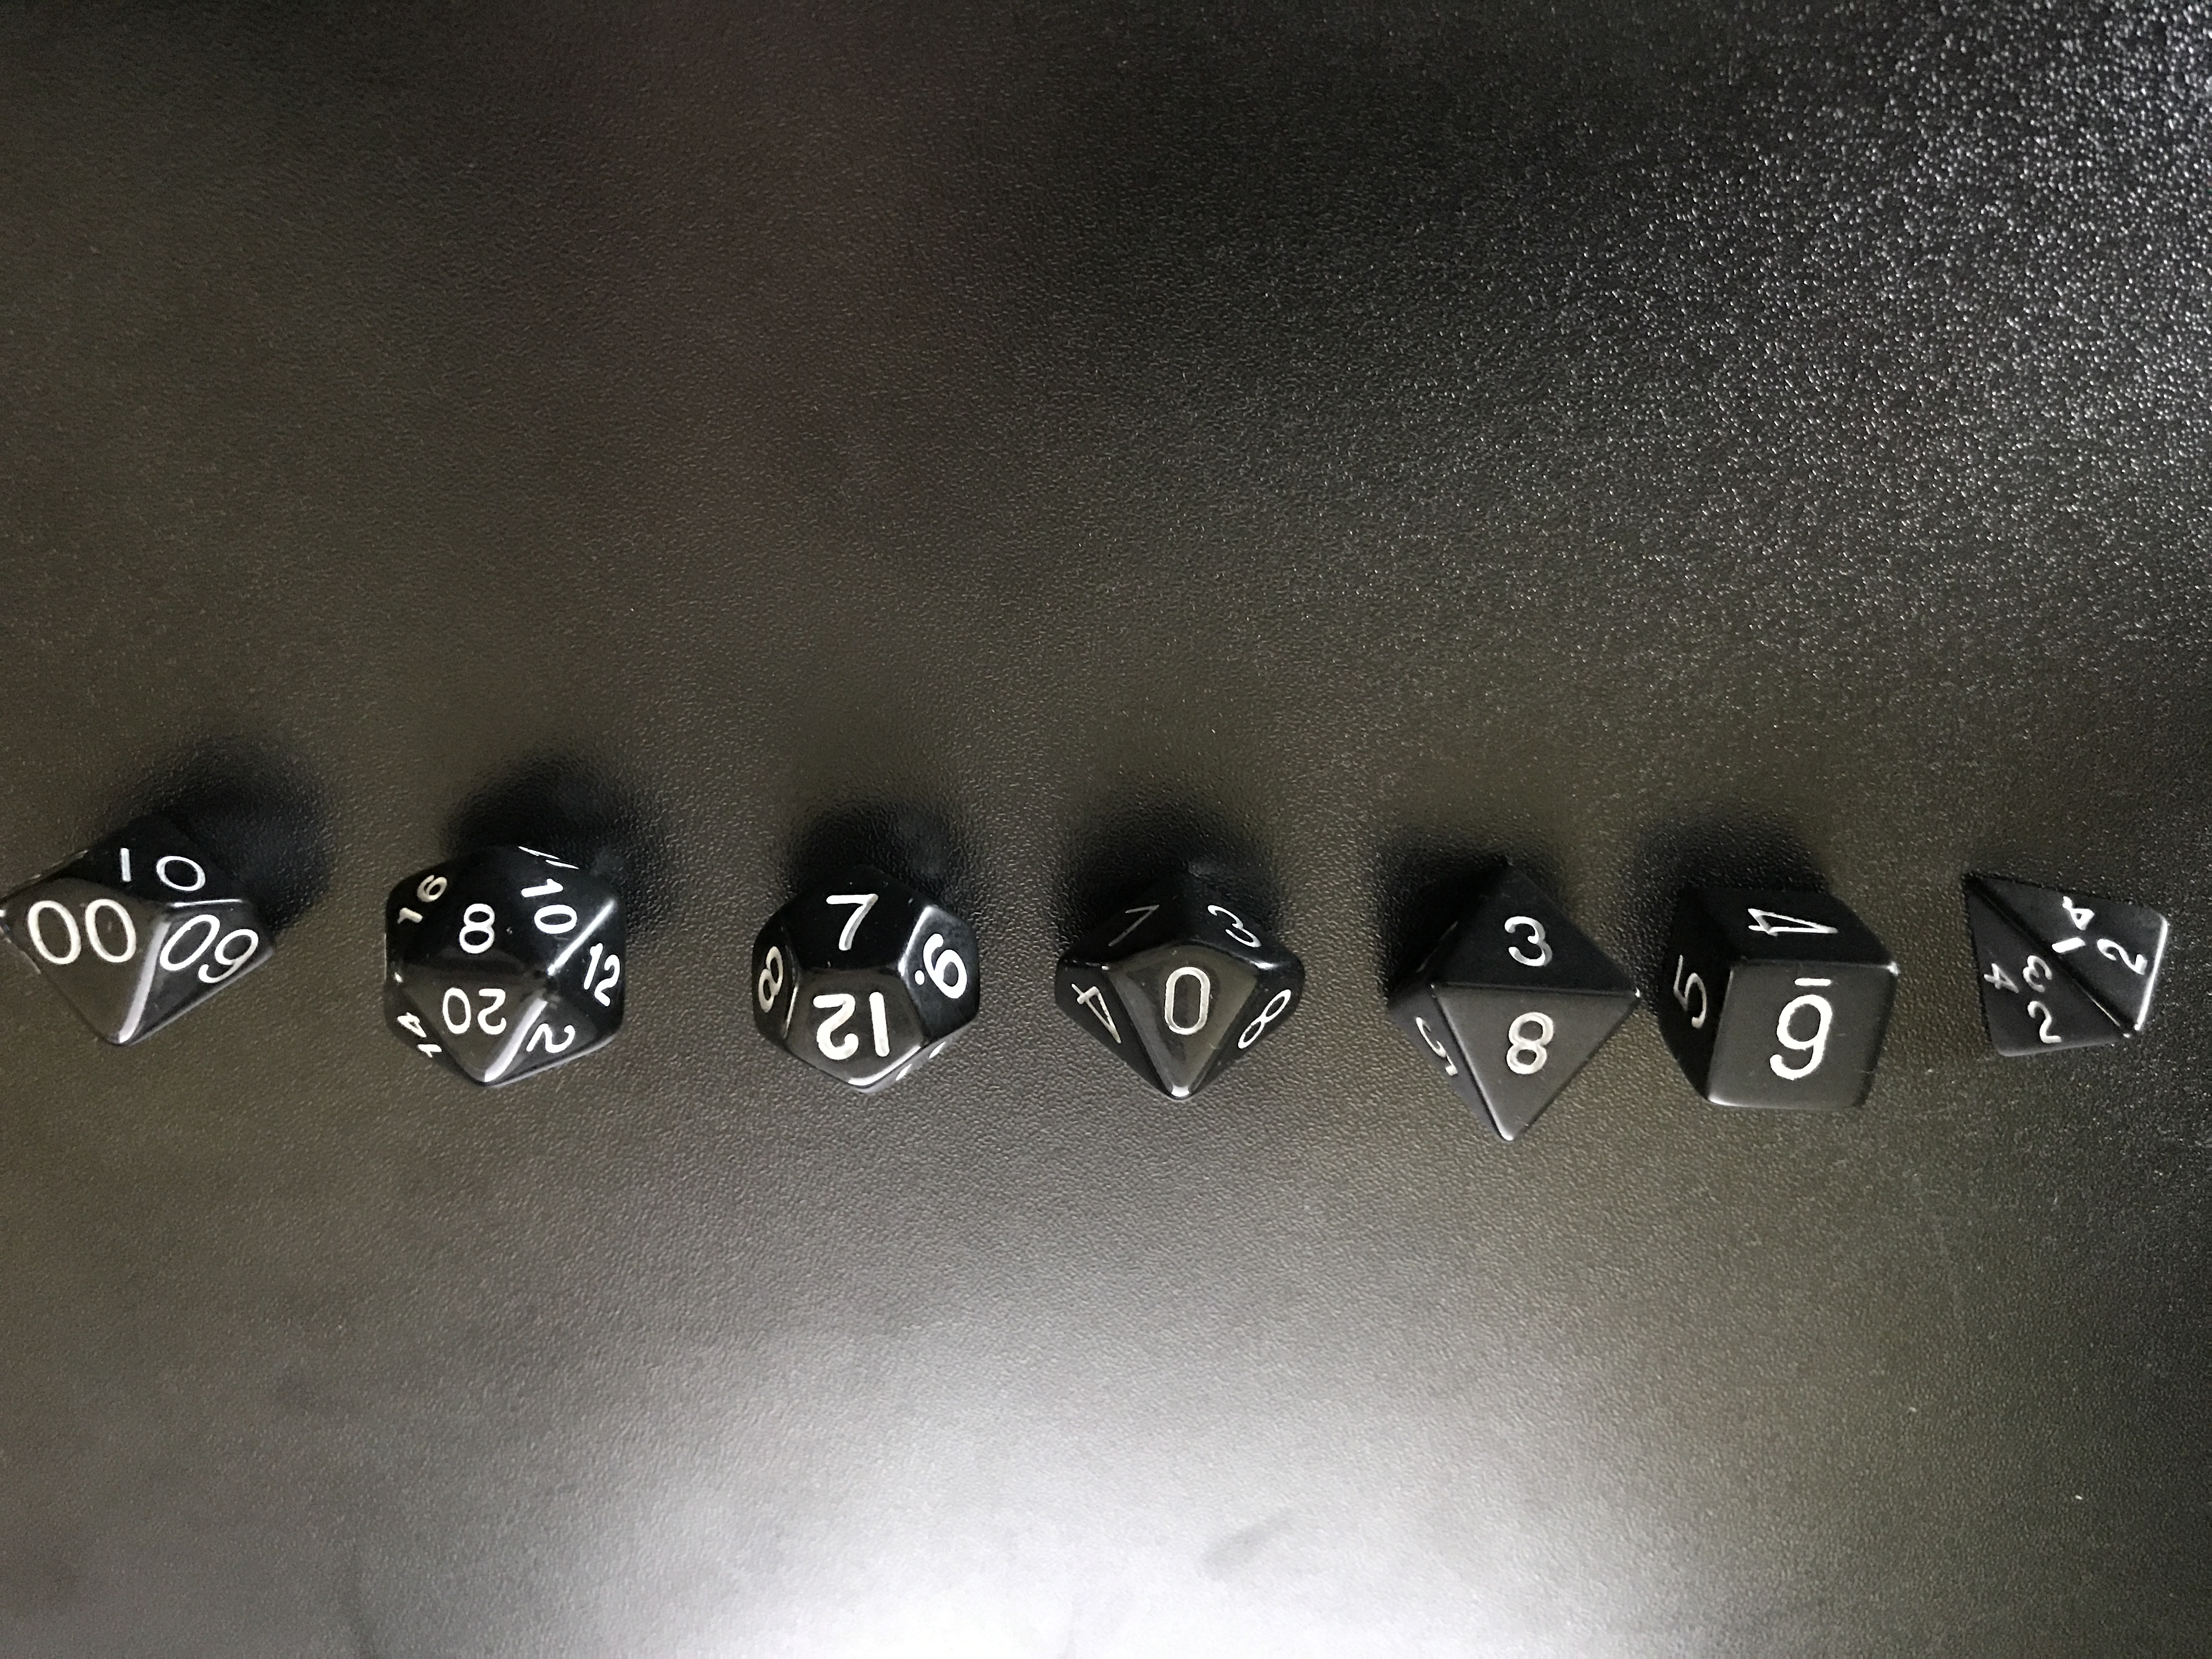
\includegraphics[width=\linewidth, height=5cm, angle=180]{DnD_Dice.jpg}
					\caption{An example set of die that was needed to play \dnd. From left to right: 4-sided, 6-sided, 8-sided, 10-sided, 12-sided, 20-sided and a 10-sided die in increments of 10s} \label{fig:DnDDice}
				\end{subfigure}
				\caption{The above two figures show the typical equipment for a \dnd \ game}
			\end{figure}
			
			Despite the complicated nature of \dnd \ the equipment that was needed to play the game was minimal. A group of players would only have needed a single set of die, a copy of the core books (\emph{Dungeon Master's Guide \citep{DMGuide}, Players Handbook and Monster Manual \citep{MonsterManual}}), a set of character sheets (1 per player), pens and paper. Everything else, such as more dice, a \emph{Dungeon Master Screen}, Campaign Books, Battle Mats and Tokens were supplementary. The die that was used for \dnd are as follows; twenty-sided, twelve-sided, two ten-sided (one in increments of ten, the other in increments of one), eight-sided, six-sided and four-sided. Figure \ref{fig:DnDLive} is an example of what a \dnd \ table might have looked like, whereas Figure \ref{fig:DnDDice} is an example of the different die used for \dnd \footnote{When discussing these die further in this paper, they will be referred to as d\emph{X} where \emph{X} is the number of sides the die has (for example the 20 sided die is referred to as \emph{d20}). The exception to this is the secondary d10 (which has increments of 10) which is referred to as the \emph{d100}.}.
			
			Throughout the campaign the party would have to face many challenges designed by the DM. These challenges might be full scale battles involving multiple powerful enemies and allies, to small scale skirmishes between only a handful of characters. Alternatively challenges could be a battle of the wills where the party have to negotiate themselves out of a tight situation with the law to passing through a magical trap set by an ancient being in order to acquire an item of treasure. The effectiveness in which the party would handle these situations are decided through a simple mathematical system. 
			
			Every character within a \dnd \ world had a set of \emph{attributes} that would dictate how that character interacted with the environment around them. These attributes are; \emph{strength}, \emph{dexterity}, \emph{constitution}, \emph{intelligence}, \emph{wisdom} and \emph{charisma} (more details of these attributes are available in Appendix \ref{app:worked-example}). These attributes were rated between 1 and 20, with 20 being the highest a character could achieve without magical means. The score would be divided by 10, rounding up to the nearest whole number, creating an \emph{ability modifier} which would be applied to the role a dice (this number could be negative) If a character was highly skilled in a particular task, then a \emph{proficiency bonus} would also be applied. This calculation is summarised in the below equation \ref{eq:skill-check}. 
			
			\begin{equation} \label{eq:skill-check}
			skill \ check = d20 + ability \ modifier + proficiency \ bonus
			\end{equation}
			
			These skill checks allowed the players to interact with the world, via the player character, in a quantitative manner. The higher a skill check was the better that character performed in that challenge. Challenges would have a \emph{difficulty class}, an arbitrary number which indicates the level of skill (or luck in some cases) needed to perform that task. If the challenge was to strike an enemy, it would be easier to wound someone wearing no armour than it was to wound a skilled warrior in plate armour. 
			
			Winning a game of \dnd \ was no simple manner either, as there were no set win conditions. It depended entirely on the campaign that was being ran by the DM. A typical example might be that the party were a group of loyalists who were tasked with overthrowing a usurper and restoring the rightful monarch to the throne. That party would \emph{win} where they to do so, however the objectives might change where the party to learn of some new, unsavoury, information about their beloved monarch. A campaign might end without achieving the original goal, or shorter campaigns may end with the start of a new story for the party. It all depended on the attitude of the players towards the game.
			
			For a short, worked example of \dnd \ please refer to Appendix \ref{app:worked-example}, where a scenario is explored and explained. 
			
			\subsubsection{How does a Dungeon Master differ from a Player?} \label{sec:dm-vs-player}
			In Section \ref{sec:what-dnd}, we explored some of the principles that gave \dnd \ life, however the most important principle to the \Codex \ app was the difference between a DMs and Players. As briefly explained above, a DM was a member of the group who would control the narrative of the campaign and dictate what was occurring during each session. Whilst the DM may write the campaign narrative themselves and would of had a great deal of control over it, they would not own the story. That belong to the group as a whole. Player input during the sessions shaped the world and story as the party progressed through the campaign, forming relationships with characters that the DM portrayed. 
			
			It was the responsibility of a DM that the party was enjoying the campaign, narrative and challenges. As a result the DM would had to have known every intricacy of the world at any given time, or be able to improvise when they did not know the answer. Only a DM could bring a world to life. Therefore the amount of information that a DM would have to deal with would have been immense. Every DM would have a folder (either physical or digital) full of notes on places, people and events that resided within the DMs world. This folder would not only contain the events of the past, but plans for the future. Skilled DMs would rely on their folder more than any other resource during a session to ensure the correct reaction to party input. The maintenance of a DM folder was costly in both time and effort \citep{GMTips}. Whilst there was no definitive time spent in order to prepare for a session, DMs could easily spend over ten hours a week planning their \dnd \ campaign \citep{DungeonMaster}. 
			
			However, DMs were part of the game just like the players were. \dnd \ was never the party against the DM, instead it was a symbiotic relationship where they would explore the world together and share the experience. Whilst a DM knew what was planned to happen next, it was decided by the players if what actually occurred. 
				
			\subsubsection{Why was the \Codex \ app developed?} \label{sec:why-codex}
			As mentioned in Section \ref{sec:context}, \Codex \ began as personal project for the author of this paper. The original functionality of the app was to be a platform for tracking combat during games of \dnd. Since then the functionality has grown to include a note taking system and several other minor features that will be discussed in Section \ref{sec:dev-and-imp}. Whilst there are several other systems (explored Section \ref{sec:other-dnd-apps}) that assist a DM, they often only perform one task. The \Codex \ app aimed to be the assistance app for DMs by possessing a wide range of functionality. 
			
			DMs spend a lot of time and effort in running their games of \dnd (as discussed in Section \ref{sec:dm-vs-player}). The \Codex \ app attempted to remove some of the more laborious tasks from DMs and put more enjoyment into the game by removing some of the pressure. As of the time of writing, the principle functionality the \Codex \ app was to track combat and provide an interactive database of information about the world for quick reference.

	\section{Related Work} \label{sec:related}
	In this Section we will explore the work that was pertinent to the \Codex \ project. We will have a greater appreciation of the \Codex \ app, by evaluating the similar systems available at the time of writing, and and gain an understanding of the Software Engineering discipline in addition to the Web-App architecture through the review of academic works.
	
		\subsection{Dungeon and Dragons Apps} \label{sec:other-dnd-apps}
		At the time writing, there were several applications that existed to assist in the running of \dnd. These apps had varying levels of functionality, however they differed from the \Codex \ app. For example, the official \dnd \ Beyond app \citep{dnd-beyond} (discussed further in Section \ref{sec:dnd-beyond}), had a huge range of functionality including digital character sheets and a quick reference database. This service is aimed towards the players of the game, not towards the DMs, therefore \dnd \ Beyond does not support session planning and encounter generation to the same level as the \Codex \ app.
		
			\subsubsection{\dnd \ Beyond} \label{sec:dnd-beyond}
			
			\subsubsection{Roll20} \label{sec:roll20}
			
			\subsubsection{ProD\&D Dungeon Generator} \label{sec:prodnd}
	
		\subsection{Software Engineering} \label{sec:software-eng}
		The \Codex \ project was not only the development of a web-app based around the \dnd \ game. It was the evaluation and examination of an agile single developer software engineering methodology. In order to perform this evaluation, we must first have an understanding for the Software Engineering Discipline (see Section \ref{sec:what-se}). From there we will learn about the Agile principles and how they changed Software Engineering (see Section \ref{sec:what-agile}). Finally, we will examine two potential single developer agile methodologies which would be compatible with the development of the \Codex \ app (see Sections \ref{sec:agile-solo} and \ref{sec:xp-for-one}). 
			
			\subsubsection{What is Software Engineering?} \label{sec:what-se}
			boo
				
			\subsubsection{What is Agile?} \label{sec:what-agile}
			boo
			
			\subsubsection{Agile Solo} \label{sec:agile-solo}
			boo
			
			\subsubsection{XP for One} \label{sec:xp-for-one}
			boo
			
		\subsection{Web App Technology} \label{sec:web-app}
		The \Codex \ app was designed to be a Web Application (web-app). In this Section we will learn what a web-app is and how it differs from the traditional website and application (see Section \ref{sec:what-web-app}). ReactJS is a popular library for the JavaScript programming language that was developed specifically to develop web-apps. Due to the popularity and availability of supplementary materials of ReactJS, it was selected to be the principle programming language for the \Codex App (see Section \ref{sec:react-js}). Semantic UI (User Interface) is a package developed for ReactJS systems, which would allow developers to quickly create professional UI for web-apps and was used in the development of the \Codex \ app (see Section \ref{sec:semantic-ui}). Finally in this Section we will look at how Databases would operate within web-apps (see Section \ref{sec:databases}). 
		
			\subsubsection{What is a Web App?} \label{sec:what-web-app}
			Web-apps were differentiated from the traditional website in that they could be easily ported onto mobile devices as a separated application on that device. Which can still be accessed through web addresses.
				
			\subsubsection{ReactJS} \label{sec:react-js}
			boo
			
			\subsubsection{Semantic UI} \label{sec:semantic-ui}
			boo
			
			\subsubsection{Databases within Web Apps} \label{sec:databases}
			boo
			
	\section{Development and Implementation} \label{sec:dev-and-imp}
	boo
	
		\subsection{Using Agile Solo} \label{sec:use-agile-solo}
		boo
			
		\subsection{Design} \label{sec:design}
		boo
		
		\subsection{Development Observations} \label{sec:dev-obs}
		boo
		
	\section{Outcome of the \Codex \ project} \label{sec:outcomes}
	boo
	
		\subsection{Development of \Codex} \label{sec:codex-development}
		boo
			
		\subsection{Effectiveness of Agile Solo} \label{sec:agile-solo-effect}
		boo	
		
		\subsection{Feedback on the \Codex \ app} \label{sec:feedback}
		boo
		
	\section{Evaluation of \Codex} \label{sec:evaluation}
	boo
	
		\subsection{Development Issues} \label{sec:dev-eval}
		boo
			
		\subsection{Agile Solo Evaluation} \label{sec:agile-solo-eval}
		boo
			
	\section{Conclusions} \label{sec:conclusions}
	The \Codex \ project was to software engineer a progressive web app built in ReactJS, using an agile methodology. The principle challenge of \Codex \ was that, unlike the majority of software engineering project, there was only one developer. Agile methodologies are designed to be used by a group or groups of developers, with designated roles for individuals within the team. As part of the preparation for \Codex, a single developer methodology had to be found, these were \AgileSolo \ and \emph{XP for One}. Agile Solo was selected to be the principle methodology for the development of \Codex. 
	
		\subsection{Agile Solo} \label{sec:agile-solo-conc}
		Agile Solo, as described in Section \ref{sec:agile-solo}, is a methodology that was developed because there was no Agile development methodology designed for solo developer projects. The purpose of a software engineering methodology is to provide a platform to assist with time and task management for a project, in that respect we need to have a certain amount of discipline from the developer when applying a methodology to a project. [It was this discipline that came a critical issue with a solo developer project. When working in a team, each developer is held accountable by the rest of the team. But in solo developer projects no one is holding the developer to account, with the notable exception of a supervisor when present.] However, Agile Solo functioned without flaw when implemented as the original author described. This is evidenced by the project journal, which can be found in the \Codex \ portfolio, where there are numerous entries that prove the following of Agile Solo. The work that was allocated each cycle was achieved and any issues in time spent of that work was down to an incorrect estimation during the allocation process.
		
		In summary, Agile Solo has proven to be a highly effective and accurate methodology for solo developer projects. The methodology proposed in 2011 by Nyst{\"o}m does not need any alterations as far as \Codex \ is concerned.  
		
		\subsection{\Codex} \label{sec:codex-conc}
		\begin{itemize}
			\item The Codex app was a large ambitious project with many complicated features
			\item Developed in a new language to the developer
			\item Developer achieved a working system that provided the core functionality of the app that met the requirements
			\item Many advanced features are easily integrated with more work
			\item Project was not a success as all features were not completed, however it was not a failure as the requirements were satisfied
			\item Therefore the \Codex \ app is a challenged project in accordance with the Standish Group Chaos Report classifications
		\end{itemize}
	
	\clearpage
	\appendix
	
	\section{\Codex \ Gantt Chart} \label{app:gantt}
	
	\begin{cmpfigure}{\Codex \ Gantt Chart, outlining the major tasks and deliverables\label{pplan}}
		\begin{sideways}
			\newganttchartelement{voidbar}{
				voidbar/.style={draw=black, top color=black!25, bottom color=black!23
			}}
			\begin{ganttchart}[y unit chart = 0.75cm, y unit title = 0.75cm, x unit=0.45cm, vgrid, title label font=\scriptsize,
				canvas/.style={draw=black, dotted}]{1}{34}
				\gantttitle{Project schedule shown for e-vision week numbers
					and semester week numbers}{34} \\
				
				\gantttitlelist{8,...,41}{1}\\
				\gantttitlelist{1,...,12}{1} \gantttitle{CB}{4}
				\gantttitlelist{1,...,9}{1} \gantttitle{EB}{4}
				\gantttitlelist{10,...,14}{1}\\
				
				%The elements, bars and milestones, are identified as elem0, elem1, etc.
				\ganttbar{Project Proposal}{1}{2} \\        		%elem0  
				\ganttbar{Literature Review}{2}{5} \\      			%elem1 
				\ganttmilestone{Literature Review Finished}{5} \\	%elem2
				\ganttbar{Design Doc. Iteration 1}{4}{8} \\ 		%elem3
				\ganttbar{Development Iteration 1}{9}{11} \\		%elem4
				\ganttbar{Progress Report}{11}{12} 					%elem5
				\ganttmilestone{}{12} \\							%elem6
				\ganttbar{Development Iteration 2}{11}{12}  		%elem7
				%week 1 of semester 2 is the 17th week in schedule 
				\ganttvoidbar{}{13}{16} \\                     		%elem8
				\ganttbar{Final Report Writing 1}{17}{19} 	        %elem9
				\ganttmilestone{}{19} \\							%elem10
				\ganttbar{Design Doc. Iteration 2}{19}{20} \\      	%elem11
				\ganttbar{Development Iteration 3}{21}{26} \\		%elem12
				\ganttbar{Testing}{24}{26} \\						%elem13
				\ganttmilestone{Code Delivery}{26} \\       		%elem14
				\ganttbar{Final Report Writing 2}{27}{30} \\  		%elem15
				\ganttbar{Inspection preparation}{31}{34}   		%elem16
				
				\ganttlink{elem0}{elem1} \ganttlink{elem1}{elem2} \ganttlink{elem2}{elem3}
				\ganttlink{elem3}{elem4} \ganttlink{elem4}{elem5} \ganttlink{elem5}{elem6}
				\ganttlink{elem5}{elem7} \ganttlink{elem8}{elem9} \ganttlink{elem10}{elem11}
				\ganttlink{elem11}{elem12} \ganttlink{elem12}{elem13} 
				\ganttlink{elem13}{elem14} \ganttlink{elem14}{elem15}
				\ganttlink{elem15}{elem16}
			\end{ganttchart}
		\end{sideways}
	\end{cmpfigure}	
	
	\section{Worked Example of Dungeons and Dragons} \label{app:worked-example}
	Strength dictates how strong a character is and would be used in determining physical challenges of raw power. Dexterity indicates the precision a character would move with, and can be used for sneaking and dodging actions. Constitution would reflect the tenacity of a character, this attribute dictates the number of \emph{life points} a character would have and how resistant to disease he/she is. Intelligence can be used to investigate a crime scene and would typically indicate how smart a character is. Characters with a high wisdom attribute would notice things quickly and are more in tune with the spiritual. Finally, the Charisma attribute would dictate how sociable a character might be, determining that characters effectiveness at persuasion and deception. 
	
	\clearpage	
	\bibliography{projectbib}
\end{document}
% EOF Document